\documentclass[a4paper,11pt]{article}

\usepackage{graphicx}
\usepackage{natbib}
\usepackage[utf8]{inputenc}
\usepackage{tabularx}
\usepackage{hyperref}
\usepackage{color}
\usepackage[usenames,dvipsnames,svgnames,table]{xcolor}
% \usepackage{mathptmx} % Times New Roman

\setlength{\topmargin}{-0.4mm} % (1in=25.4mm)-0.4mm=25mm
\setlength{\textheight}{243.119mm} % 297mm-40mm-10mm-(11pt=3.881mm)=
\setlength{\oddsidemargin}{-0.4mm} % (1in=25.4mm)-0.4mm=25mm<
\setlength{\textwidth}{160mm} % 210mm-50mm=160mm
\setlength{\headheight}{0mm}
\setlength{\headsep}{0mm}
\setlength{\footskip}{15mm}

\providecommand*{\note}[1]{\small \textcolor{RoyalBlue}{\begin{minipage}{\textwidth}{#1}\end{minipage}}}

% --------------------------------------------------------------

\providecommand*{\ShortTitle}{Modern voluntary Health Care System}
\providecommand*{\FullTitle}{The influence of gamification on the willingness to live healthy}

% --------------------------------------------------------------

\title{\textbf{\sffamily\Huge \ShortTitle}\\ 
{\textbf{\sffamily\Large \FullTitle}}
\vspace{1cm}}

\author{
{\em 188.407: Management von Software Projekten} \vspace{1cm} \\
Group: 12\bigskip \\
Dominik Oberhumer \\ {\small 1025454, 033 534, \href{mailto:e1025454@student.tuwien.ac.at}{e1025454@student.tuwien.ac.at}}\\
Gerhard Schraml \\ {\small 0728067, 033 534, \href{mailto:e0728067@student.tuwien.ac.at}{e0728067@student.tuwien.ac.at}}\\
Johannes Kurz \\ {\small 0727957, 033 534, \href{mailto:e0727957@student.tuwien.ac.at}{e0727957@student.tuwien.ac.at}}\\
Matthias Tretter \\ {\small 0726390, 066 937,  \href{mailto:e0726390@student.tuwien.ac.at}{e0726390@student.tuwien.ac.at}}\\
Philip Messlehner \\ {\small 0728061, 066 937, \href{mailto:e0728061@student.tuwien.ac.at}{e0728061@student.tuwien.ac.at}}\\
\vspace{4cm}
}

\begin{document}

\begin{titlepage}
\maketitle

\end{titlepage}

% --------------------------------------------------------------

\thispagestyle{empty}
\tableofcontents
\pagebreak

\setcounter{page}{1}


% --------------------------------------------------------------

%\note{
%\textbf{Formal constraints}
%\begin{itemize}
%\item	  Font: Times New Roman oder Computer Modern (\LaTeX default)
%\item    Fontsize: 11pt
%\item     Single line spacing
%\item     Margins: 2.5cm side and top/bottom
%\item     \fbox{Language: ENGLISH}
%\item    The proposal template should be filled incrementally. I.e., at the end there should be a full project proposal in a single PDF file.
%\end{itemize}
%\textbf{Available templates}
%\begin{itemize}
%\item     Proposal (mswp-proposal.tex)
%\item     Costs (costs.xls, costs.ods)
%\end{itemize}
%\textbf{Supplemental material}
%\begin{itemize}
%\item     FWF salary scheme (\href{http://www.fwf.ac.at/de/projects/personalkostensaetze.html}%{http://www.fwf.ac.at/de/projects/personalkostensaetze.html})
%\item     Travel cost regulation (\href{http://www.fwf.ac.at/de/faq/reisegebuehrenvorschrift.html}{http://www.fwf.ac.at/de/faq/reisegebuehrenvorschrift.html})
%\item     Ethical issues form (ethical-issues.rtf)
%\end{itemize}
%}
%\pagebreak

% --------------------------------------------------------------
\section{Synopsis}
\label{sect:synopsis}

%\note{
%\begin{itemize}
%	\item {\em Length: 1-2 pages}
%	\item Concise presentation of the scientific proposal, with particular attention to the ground-breaking nature of the research project, which will allow to assess the feasibility of the outlined scientific approach. 
%	\item WHY would you like to do WHAT, HOW would you like to do it and what are the expected RESULTS?
%	\item Short description of project idea.
%	\item Short description of problem / situation.
%	\item What makes it an interesting endeavor?
%	\item Why should somebody care?
%	\item Very short cost-benefit description (what are potential benefits that make them worth the costs of the project?).
%	\item Who are the beneficiaries of the results?
%	\item Problem classification (to which scientific area does the project belong?; is it basic or applied research?)
%	\item Constraints
%	\begin{itemize}
%		\item     The project must have an extent that demands to handle it as a project including project organization.  (No 2 person pieces; no 150 person-year efforts)
%		\item     Software development should be part of the project. (But not its only content or scientific contribution.)
%		\item     The project should be interesting and meaningful.
%		\item     {\em Your creativity is called for!!}
%	\end{itemize}
%\end{itemize}
%}

The ultimate goal of the Modern Voluntary Health-Care System is to create and publish a new form of an e-health system that encourages users to live healthy. This platform is based on a bonus malus system to give users an easy understandable overview on how healthy they live and how they compare to others. \\

The project is split in both a scientific and an engineering part. The scientific part aims at searching for technical methods to encourage people to live healthier and generating knowledge of the influence of gamification on the willingness of people to live healthy. From a scientific perspective it is interesting to see how well-known methods like gamification and competition can be used to motivate people to live and stay healthy.

For this purpose we try to evaluate and answer some questions, such as:

\begin{itemize}
\item How can people, by technical means, be subconsciously forced to change their ways and daily routines?
\item Is there a way to achieve practical improvements in peoples health by providing a playful approach to do so?
\item Are those improvements comparable to e.g. consulting professionals such as nutritionists, health trainers or even doctors?
\item Does competition motivate people to stay healthy?
\end{itemize}

The knowledge generated from these tests and questions can be used as a scientific backbone on the journey to a more healthy and fit society. From a psychological perspective it's important to generate data on how gamification of all-day tasks like eating, walking and avoiding health traps can improve the attitude and willingness of people to live healthy. Combined with a modern workflow and easy tracking of health-related data by offering a mobile interface our study aims at generating new knowledge in the field of gamification through technology. Moreover the study should reveal useful information on the usability and user interface of such a system. A clunky interface and no support for automatic tracking of information ultimately means a failure of the whole system. Is is vital to generate useful and accurate data of each participant because the system stays and fails with the usefulness of the collected data. We can't force the user to manually enter each and every task he does throughout the day, we need to automate this process as much as possible and we need to integrate with other tracking systems to get access to even more data. The interface of the modern health-care system should stay out of the way of the user, it should intelligently track the information needed to generate good statistics of the habits of the participant.

Case studies including user tests in the section of human computer interaction shall lead to a basis for developing a completely innovative and ground-breaking health-care system, which brings benefits to several different parties.\\

The engineering part is split into different phases. This leads to the creation of a usable, rudimentary but integrated prototype after a short time. Nevertheless, the vision is a long-term development. For each phase it is necessary to find different partners in economy, politics, health-care and science. The partners mainly use our platform for advertisement and customer relationships, which brings benefits to them as well.

\pagebreak

Possible Partners are:
\begin{itemize}
	\item Phase 1:
		\begin{itemize}
			\item Supermarkets
			\item Fitness Centers
			\item Restaurants
			\item Doctors
		\end{itemize}
	\item Phase 2 - $"$Integrating with existing services$"$:
		\begin{itemize}
			\item Sport-Community with Tracking (e.g. Runtastic, RunKeeper, Nike Plus, ...)
			\item Other health-related tracking services (e.g. Pedometer, Weighttracking, ...)
			\item Health-related gaming platforms (e.g. Geocaching, ...)
		\end{itemize}
	\item Phase 3 - $"$A new form of health-care system$"$:
		\begin{itemize}
			\item Insurances 
			\item WHO
		\end{itemize}
\end{itemize}

When a user buys something in a partner shop the product gets registered at our platform. The system stores the information in an anonymised form and calcualates statistics based on a transparent score-schema. The user can then exchange his earned points for gifts like coupons for healthy shopping at a partner's store. Moreover the platform generates a monthly, opt-in ranking of people living in a specific area, people who register them as a group of friends or all registered people as a whole. It therefore aims at answering questions like $"$which user lives most healthy?$"$, $"$which user eats most healthy?$"$, $"$which user walks the farthest distance in a day?$"$ and similar. Partners are able to interact with the user with the use of the platform so they can selectively advertise new products of interest for the user. \\

The goals of the platform:
\begin{itemize}
\item \textbf{Improving overall health of the user}: People are getting more sensible for health-care. So they get forced to live in a healthier way. Our health care system is very expensive. The whole government should have a benefit from this platform and more healthy people. 
\item \textbf{Financial benefits for the user}: Users will be given discounts and coupon codes when buying healthy products at partner stores. 
\item \textbf{Advertisement for the partners}: For the partners the platform offers a chance to advertise their promotions. Furthermore they have the chance to give coupons to the users. With this coupon they can interact with the customer. One possible effect is a gain in customer loyalty.

\end{itemize}

\pagebreak

% --------------------------------------------------------------
\section{Introduction and problem description}
\label{sect:intro}

%\note{
%\begin{itemize}
%	\item {\em Length: 2-3 pages}
%	\item {\bf Why?}
%	\item Introduction
%	\item Context
%	\item What is the current situation?
%	\item What is the open/unresolved problem or opportunity?
%	\item Why is it a problem?
%	\item What is unknown?
%	\item What could be improved?
%	\item Explanation of fundamental terms and basic definitions.
%\end{itemize}
%}

Recent studies \citep{euobes2003} show that more and more people are getting obese these days due to an unhealthy lifestyle and way too less exercise, especially in the so called western society. Many studies and health reports in Europe and America describe the problem and show an increasing trend towards being overweight. The biggest problem in this area is that the situation is getting worse and worse. Especially children are rapidly becoming a big part of the problem, the risk of being an overweight child in the US is about 30 percent - according to the Center for Disease Control \footnote{\url{http://news.stanford.edu/news/2004/july21/med-obesity-721.html}}. Another recent study suggests that at-risk children are identifiable in their first years of life and tries to identify various risk factors \footnote{\url{http://news.stanford.edu/news/2004/july21/med-obesity-721.html}}. \\

The situation in Europe isn't any better. European studies\citep{rki2012} show, that about 23 percent of the people living in Germany are obese nowadays. In the Forbes List for the fattest nation, Austria ranks on place 52 with a fat rate of 57.1\%.\footnote{\url{http://www.forbes.com/2007/02/07/worlds-fattest-countries-forbeslife-cx_ls_0208worldfat_3.html}}. Figure \ref{fig:obese_in_eu_pdf} shows a rather recent statistic of the situation in 25 European countries, divided by sex. 

Being overweight affects your life in a lot of ways. From today's point of view overweight people are less attractive than others, have less success and and are more likely to be the victims of day-to-day discrimination \citep{carr05}. Moreover obesity can lead to very serious health problems like hypertension, asthma, diabetes and other cardiovascular problems.  \\

\begin{figure}[tb]
	\centering
	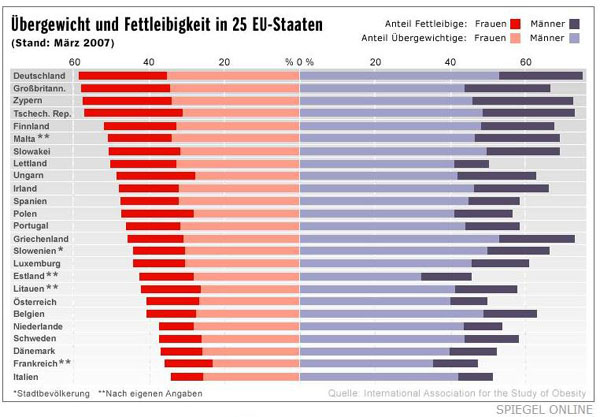
\includegraphics[width=1\textwidth]{images/introduction/1.jpg}
	\caption{Obese in the EU}
	\label{fig:obese_in_eu_pdf}
\end{figure}

One reason for the negative trend of childhood overweight are bad role models. Parents living an unhealthy lifestyle affect and influence their children. With increased age it gets harder to get in shape, the goal should be to teach children at young ages how to become and stay fit. In the future this negative trend will lead to an increased financial claim in our health care system - more and more people need expensive health treatments because of diseases caused by being obese over the years.  \\

The only way to stop this trend and to reduce the costs for health treatment is to live healthier today. This is the point where our modern health care system comes into play: We want to help people improving their lifestyle and staying fit by motivating them through the help of gamification and technology. Rankings against friends and neighbours as well as bonuses for reaching milestones are a vital part of our system. People shouldn't get forced to live healthy, they should do it self-motivated. We want to increase this motivation. This will eventually lead to a healthier society over time.  \\

Our goal is to make people realize how they can benefit from a healthier lifestyle. A latin quote goes as follows:

\begin{center}
	\emph{"Mens sana in corpore sano"}
\end{center}

A sound mind in a healthy body, people that are healthy feel happier. Unfortunately it is way harder to motivate people to look after themselves than it should be. One's weaker self is often blamed for becoming a so called modern couch potato. Combined with the increasing stress of today's achievement-oriented society this leads to long working hours without time for healthy meals or exercises. Most people ignore the fact that often small changes of their habits can lead to a healthier lifestyle without having to invest hours a day for doing sports. Taking the stairs instead of the elevator, using a standing desk instead of sitting in front of the computer all day long, taking the bike to work, buying fruits and healthy meals instead of chunkfood - all these things can dramatically improve your fitness and can be easily integrated as your day-to-day routines. What's missing? The motivation to do so. People are easy to influence (in a good sense). People are driven by results they can see and by competing with people they know. People want to be better than others, naturally. People enjoy being rewarded for their efforts. We want to use these inner forces and turn them into something good, we want to use them to help people improve their lifes. \\

Overall our modern health care system should lead to lowered costs for health care in general and it might be possible to integrate the system with private insurance systems. People would see another benefit of living healthy: cheaper insurance. People like to save money. \\

This project is accompanied by a scientific study. The goal of the study is to generate relevant data on which arrangements can motivate people the most and lead to best results as well as how people interact with a modern, technology-driven health care system and how to improve these interactions. The focus hereby is on the usability of an ubiquitous health tracking system that (half-)automatically generates useful data of the habits of the participants. This data should lead to a good basis for future work on the topic. \\

% --------------------------------------------------------------
\pagebreak

\section{Project goals and deliverables}
\label{sect:goals}

%\note{
%\begin{itemize}
%	\item {\em Length: 1-2 pages}
%	\item What is the goal of the project?
%	\item Research questions
%	\begin{itemize}
%		\item 	    What are the hypotheses that are to be investigated?
%		\item 	    Main hypothesis \& sub hypotheses
%	\end{itemize}
%	\item Which results should be achieved with the project?
%	\begin{itemize}
%	    	\item 	   What will be known afterwards that is not known now?
%		\item	    What will be created that does not exist now?
%	\end{itemize}
%	\item Non-goals (What will not be part of the project? What will not be done?)
%\end{itemize}
%}

The goal of the modern health care system is to create a new form of voluntary system that motivates people to live and stay healthy. 
It is based on several pillars:

\begin{itemize}
	\item \emph{Technology}. 
	The goal of the modern health care system is to use today's possibilities to support a healthier lifestyle. Technology is often blamed as a culprit for the increasing number of unhealthy people. We want to use technology to increase the overall health of people. Currently there are several focused approaches that use technology to improve health, see \ref{sect:star}. We want to create a system that does not only track isolated parts of your health-related activities but rather creates a big picture of everything you do and therefore is much more accurate than the existing systems.
	\item \emph{Ubiqitous Computing and Usability}.
	The modern health care system should be an easy to use system that transparently integrates into ones living day while staying out of the way and minimizing the need of manual interactions. The increasing success of mobile computing was a start to a new form of computing ultimately leading to ubiquitous and pervasive computing in the future. Ubiquitous computing is a post-desktop model of human computer interaction and describes the integration of computing into everydays activities. The modern health care system should be a case study on how ubiquitous computing performs on a broader range. 
	\item \emph{Psychology}.
	The modern health care system should use and gather knowledge on what motivates people to stay in shape, especially in the field of gamification. The broad range of data generated by our system should be analyzed and evaluated to generate statistics on how gamification of everydays tasks can improve life. The game designer Jane McGonigal describes her journey from becoming suicidal to enjoying life in her TED talk \emph{The game that can give you 10 extra years of life} \footnote{\url{http://www.ted.com/talks/jane_mcgonigal_the_game_that_can_give_you_10_extra_years_of_life.html}}. She describes how turning her life into a game changed her perception of life and made her a happy person. This and other examples clearly show that gaming can have a very high impact on peoples life, with the help of the modern health care system we want to generate scientific data to prove this.
	\item \emph{Security and Privacy}.
	The increasing trend to an interconnected system and to ubiquitous and pervasive computing leads to higher risks of misuse of data. Health related data is very sensible data and therfore the modern health care system must guarantee data security and privacy from today's point of view. We need to investigate in how communication can stay private and how data can be obsfuscated without loosing the ability to generate useful statistics.
\end{itemize}

There are several research questions to be investigated:
\begin{itemize}
	\item How can tracking be automized and done transparently without the need of manual interaction?
	\item How does gamification of day-to-day tasks affect people‘s motivation?
	\item How can ubiqitous computing be used to support improving our health?
	\item How can different ecosystems be integrated into one giant, interconnected system without sacrifying security and privacy?
\end{itemize}

The main hyphotesis to be investigated in this project is in the field of usability and ubiquitous computing. We want to generate knowledge on how a tracking system that monitors your whole day can be designed without being noticable and annoying. As already stated such a system can only succeed if the generation of useful data is as automized as possible, manual entries of exercices or nutrition facts can improve the data accuracy but shouldn't be vital for a working system. \\

The focus of the modern health care system isn't to become a game and therefore to compete with other game approaches like XBox Kinect or the Nintendo Wii. The main goal of these devices is to be a gaming platform, exercising while playing is a secondary factor that is to a great extent used for marketing reasons. Furthermore the modern health care system is no phychological study. The knowledge generated in this area is a side-product and not the main focus and the evaluation of the generated data is not part of the project. We also do not want to create an advertisement platform that can be (ab)used by our partners to spam our users. We do offer targeted ads, but only to a certain extend to be able to gain the interest of more partners in the industry.

% --------------------------------------------------------------
\section{Scientific relevance and innovative aspects}
\label{sect:relevance}

%\note{
%\begin{itemize}
%\item {\em Length: 1-2 pages}
%\item Why is the project scientifically interesting?
%\item Did others point out that this is an open question?
%\item What are the innovative aspects that make it interesting?
%\item How could the project break new ground scientifically?
%\item To what extent are the objectives ambitious and beyond the state of the art (e.g. novel concepts and approaches or development across disciplines)?
%\end{itemize}
%}

\subsection{Scientifical point of view}
Using gamification as a motivational factor isn‘t new, there are several systems and successful gamifications like $"Foursquare"$ \footnote{\url{https://foursquare.com/about/}} on the market. See section \ref{sect:star} for a list of other systems using gamification in a health-related environment. The modern health care system is scientifically interesting because it combines several well-known approaches into a new interconnected system and it is unknown if and how such a system can work. There is a high scientific potential in our idea because it combines many of already given approaches with existing infrastructure and organizations. The modern health care system is on the one hand a psychological study on how gamification of everydays tasks can influence peoples behaviour, on the other hand it tries to gather new knowledge in the field of ubiquitous computing, usability and security/privacy. There are several questions we try to answer, see section \ref{sect:goals} for an exhaustive list. \\

It is already known that gamification, achievements and rankings can boost people's motivation. The questions we try to answer are whether gamification of simple tasks can lead to a long-term improvement of peoples attitude towards health. By using several sources for tracking we can gather more data than any other system already on the market and can therefore generate much more accurate data that is needed to answer those questions. The term \emph{ubiquitous computing} was first mentioned by Mark Weiser in 1988 and was shaped in his paper \emph{The computer for the 21st century} \cite{weiser99}. Since then ubiquitous computing became a trending form of computing which we believe will play a more and more important role in the future. The modern health care system tries to make use of ubiquitous computing in a broad range and therefore tries to push the integration of computing in day-to-day tasks and this new form of human computer interaction. By using an integrated system for health tracking on such a broad range ubiquitous computing can be pushed to its limits, since we need to track data from several forms of sources and sensors and this from a statistically relevant number of people. \\

\subsection{Open questions}
The game designer and scientist Jane McGonigal, once suffering from depression herself, investigates in several research projects and studies on how gamification can improve people's life and happiness \footnote{\url{http://janemcgonigal.com/learn-me/}}. For this purpose she once created a game SuperBetter to treat herself, leading to the founding of her company SuperBetter Labs. Her experiments show that habits learned during playing a game with real world content can influence people‘s behaviour even after the game already ended. The game \emph{World without Oil} \citep{wwoil2007} is an alternate reality game to call attention to a possible future oil shortage. People playing this game showed to be more sensitive for sustainable oil usage afterwards. The open question we want to answer is whether gamification can have a similar impact on the long-term attitude of people towards living a healthy life. We want to find out which factors can lead to a success or a failure of this system and how different societies need different motivations factors. \\

Another open question we want to answer is if and how different isolated systems can be interconnected in a useful way, and whether we can infer a general approach for such a task. One important point of the interconnected data mining is to not sacrify security and privacy, while still keeping the possibility to do useful evaluations and create meaningful statistics. There are several algorithms that can be used to do privacy-preserving data mining like Partitioning, Randomization, Group Based Anonymization or special algorithms for Distributed privacy-preserving data mining \citep{agrawal2000}. We need to research which algorithms are most suitable for our needs.

Furthermore we want to investigate in the field of human computer interaction. We want to gather knowledge on how to improve the interaction between people and their mobile phones and several other pervasive computing systems they use throughout this study. Usability in the field of mobile and ubiquitous computing is still a very new scientific topic and we want to improve our knowledge about how to design systems that stay out of the way of the user.

\subsection{Innovative aspects}
%The combination of different aspects already in use like surveillance of old people living alone to achieving the daily goal of walking 1.5 kilometers or drinking 2.5 liters of water is new. In Africa there is a project to do a basic doctor consultation by SMS. The reason for this is because nothing is spread that widely other than a simple mobile phone. Going many kilometers for a checkup to the next doctor is often way to far for people with no car or the possibility to use public transportation. Approaches like this one are already rolled out for certain diseases and specialized groups (see \footnote{\url{http://derstandard.at/1345166647163/Der-Doktor-im-iPhone}}). Combining all the existing programs to one big socialized game for healthier living could even change economy.

As described in the sections above, there are many different standalone solutions/products in the area of technical-backed healthcare. Our study aims at investigating the possibility of combining them to a whole single system which would lead to a gain in additional value. For the resulting system that means, that the user should not be forced to download and install several different apps or helpers (s)he wants to use, but get provided with one single interface which allows to benefit from it at least as much as if every single application would have been used separately by the user.

Another innovative aspect is the attempt to keep the user interface as much out of the way of the user as possible. User interface design could step at a new higher level, where less commands are necessary to get more information and benefit out of the system. We want to search for and present new ground-breaking methods in user interface design for use in ubiquitous software systems.

% --------------------------------------------------------------
%\pagebreak
\section{State of the art / current knowledge}
\label{sect:star}

%\note{
%\begin{itemize}
%\item {\em Length: 2-5 pages}
%\item What results and approaches have already been presented in this or related areas?
%\item Relation to the international scientific work in the field (international status of the research)
%\item Description and critical discussion of related scientific work
%\end{itemize}
%}

Today there are several approaches to motivate people to live healthier, but most of them are just focusing on doing your regular workout and track your success or just help to have more fun doing physical activities. \\

Analyzing these current systems you can find two strategies, on one hand the gamification of healthcare (see \ref{sect:star:gamification}) and on the other hand a combination of helathcare and social engineering with special plattforms.


\subsection{Gamification of Healthcare}
\label{sect:star:gamification}
Nowadays there are several products that are using a gamification approach to motivate the user-base to do sport-activities. This technique is used in the gaming industry to sell sport and fitness games and was also part of creating new remotes and interaction possibilities to evolve the whole gaming industry.

\subsubsection{Nintendo Wii}
\label{sect:star:wii}
One of the first well-known of these systems was introduced by the japanese company called Nintendo in the year 2005 and named Nintendo Wii. This product is a typical games consol, but offered a new kind of remote called ``Wii Remote''. The shape of this remote is also highly inspired by the form of an TV remote and uses 4 infrared sensors on top of this remote which makes it possible to point on several objects presented on the TV-screen with a precision compareable to a common mouse used for personal computers. \\

The included accelerometer is the most important part of this remote which recognizes motions and rotations of the remote and lets users play their games in a very funny and highly interactive way. \\

Another additional input device for the Nintendo Wii is called ``Wii Balance Board'' (see \ref{fig:wiiboard}), which users have to place on the floor in front of the games console. The users have to stand right on top of this board and are able to control the game by switching their weight from one side to the other side.
For user feedback they also included speakers and vibration sensors into the Wii Remote. \\

\begin{figure}[ht]
\begin{center}
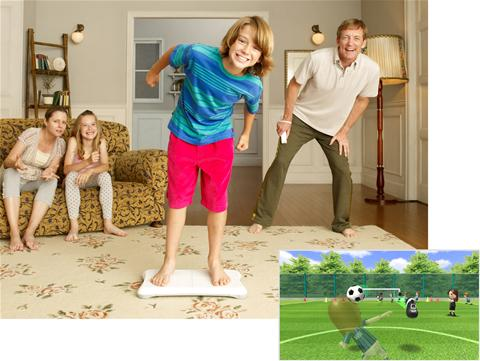
\includegraphics[width=12cm]{images/stateoftheart/wiiboard.jpg}
\caption{Wii Balance Board in action}
\label{fig:wiiboard}
\end{center}
\end{figure}

All these devices are connected via Bluetooth with the Console and are heavy used by sport and fitness games. Some rehabiliation center are using these consoles to gamify the process and making workouts more interesting. These rehabilitation centers were also observed and analyzed in medical studies showing, that patients have more fun doing their daily workout and training and also getting back to a normal physical condition more quickly. \\

Games using these features are e.g. ``Yoga'', EA Sports ``Active 2'' or the game compilation ``Wii Sports''. \\

\subsubsection{Xbox 360 and Kinect}
\label{sect:star:kinect}
Microsoft also introduced an additional remote for their Xbox 360 in the year 2010 called ``Kinect''. Kinect is working with a different Approach than Wii Remote. It's like a camera placed in front of the TV capturing the users and working with 3D motion sensor, facial recognition and voice recognition (see \ref{fig:kinect}). These facts lead to one big advantage compared to Nintendos remote: the user do not have to hald a remote in his hand and therefore the user isn't constrained within his motions and movements. \\

\begin{figure}[ht]
\begin{center}
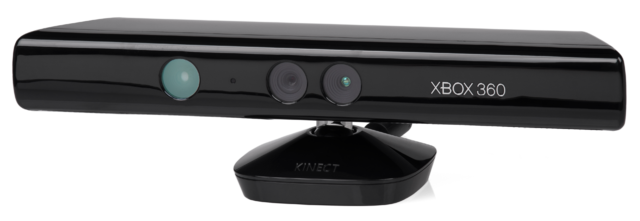
\includegraphics[width=12cm]{images/stateoftheart/kinect.png}
\caption{Microsofts Kinect remote}
\label{fig:kinect}
\end{center}
\end{figure}

Microsoft also offers a SDK and Developement ToolKit to allow programmers to build their own Kinect games or application. One of these experiements was build at the University of Minnesota and its goal was to measure or detect diseases like autism. It's also possible to connect a Kinect remote to a Windows PC which makes it easier to run such applications used in an scientific area.

\subsubsection{Playstations Remotes Eye and Move}
\label{sect:star:eyemove}
Sony also introduced in the year 2007 and 2009 two remotes, very similar to the previous described remtoes from Microsoft and Nintendo.

Playstation Eye is very similar to Xbox Kinect, offering a camera and microphone to capture the users motions and voice.
Playstation Move is an Wii Remote like remote with an additonal orb which can change the color to give additonal feedback to the user and is used as anchor point for the Playsstation Eye to recognize the movements. (see \ref{fig:playstationeyeandmove})

\begin{figure}[ht]
\begin{center}
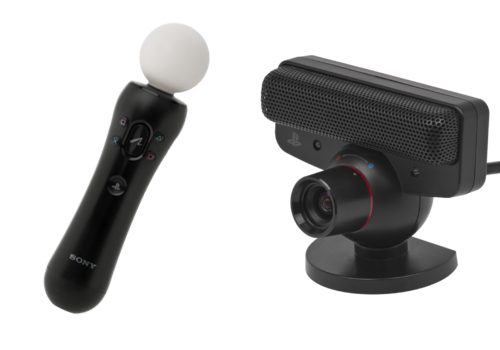
\includegraphics[width=12cm]{images/stateoftheart/playstationeyeandmove.png}
\caption{Playstation Move and Playstation Eye}
\label{fig:playstationeyeandmove}
\end{center}
\end{figure}

\pagebreak

\subsection{Socialisation of Healthcare}
\label{sect:star:social}
Another way of motivating people to live healthier and doing their regular workout is to add a social component to the expierence of making sport. The goal of this approach is to create a social network where you can track your own success and compare it to the progress of your friends. This area combines knowledge from psychology, social studies and the corresponding behaviour of human beings reacting to such social structures like social networks.

\subsubsection{Introducing RunKeeper}
\label{sect:star:runkeeper}
RunKeeper was created several years ago and started as a simple tracking plattform to track your runs. It works with several smartphones and uses their GPS sensor to track speed, distance, elevation and other things of a run.

In addition they build a website where you can see your previous runs on a map and give you overview of your last activities with monthly stats (see \ref{fig:runkeeper}).

\begin{figure}[ht]
\begin{center}
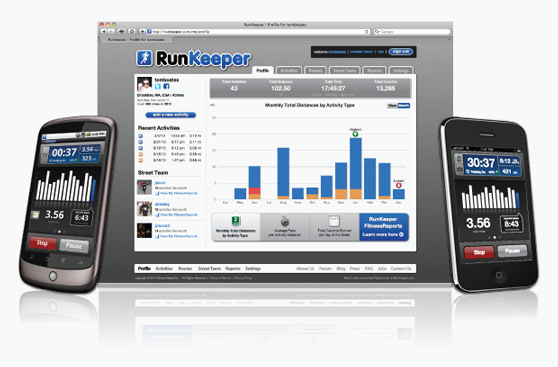
\includegraphics[width=12cm]{images/stateoftheart/runkeeper.jpg}
\caption{RunKeeper website and mobile clients}
\label{fig:runkeeper}
\end{center}
\end{figure}

\paragraph{Social aspects:} The next step was to add social features to their plattforms to make this service more intersting for their users. They introduced a route-sharing feature, which makes it possible to find interesting routes near you posted by other runners. To get in contact with these people they introduced the so called Street Team to see the activities from your friends and match against each other, a simple way to gamify your daily workout.

\paragraph{Enhance the plattform:} RunKeeper also introduces some other features to motivate the users even more to do their workout. One of these was the ability to set goals on a monthly based, like total distance or furthest run, etc. \\

They also thought how to make this plattform a little bit more profitable and released a new way to manage your training with this plattform, called ``Training Plans''. You can subscribe to these plans after paying a small fee and attend a class. The plans are created from professional trainers and have different goals, e.g. complete a 10 kilometres run within 50 minutes. The users track their run to the classes and are allowed and welcome to spread their success within the class with their classmates.

\paragraph{The look over the rim of a tea cup:} RunKeeper tried to expand their offer to cover more bases. First step was to include more different sports to allow cycler or swimmer to track their activities too. \\

Offering sport equipment to track your heart rate or your body weight and body fat were another steps in this direction to track more mesaurement parameter to observe the users health status. \\

In their blog they are spreading really nice success stories about people losing a lot of weight because of the motivitaion they got from RunKeepers apps, plattform and equipement. \\

HealthGraph is another plattform they are hosting which focuses more on the social aspects and this system is covering even more health parameter than the original RunKeeper website, but this plattform is still in kind of a beta mode.

To catch even more ideas and possibilites they also released an SDK to integrate RunKeeper into other apps and allow other plattform to use these collected data. \\

\subsubsection{Similar Plattforms}
\label{sect:star:competitors}
There are several other plattforms tracking your sport activities, a lot of them do not offer that many features as RunKeeper does, do not have that many users, or do not follow such an intense social approach.

\begin{itemize}
	\item \textbf{Runtastic:} This is a very similar system like RunKeeper but also had a lot of success during the last few years. The company is situated in Linz in Austria and expanded their user based all over the world. A lot of people switched from RunKeeper to Runtastic because of several individual reasons (e.g. design, user-base, etc.). \\
	\item \textbf{Nike+:} Nike also startet with a tracking service for runners, but they used another sport equipment to track the distance of your run. The user had to place these small sensor on one of his shoes and this sensore tracked your step like a step counter and calculated your run distance.
	
	They also began to work on an app and introduce new features and also selling their combined sport equpements like gears and so on. Also the social aspect became more and more important in their system.
	
	One big advantage is the use of Xboxs Kinect which not only combine these two plattforms but also combine the two strategies of gamification and socialisation. \\
	\item \textbf{Other plattforms introduced by several sport equipment manufactors:} Other manufactors like Polar also introduced their own plattforms but have problems to reach a big user-base. They tried to jump on this movement made by plattforms like RunKeeper or Runtastic, but couldn't get that much success with their systems, although they have a lot of success with their equipment.
\end{itemize}

\pagebreak

\subsection{Approach of this Project}
This project does not follow the same approach as the above mentioned Social Platforms or Game Consoles.

Both mentioned approaches are combining their platform or consoles as tool to give people motiviation to do their workout, but do not cover other health aspecets as diet or food at all. \\

The goal of this project is to make people live healthier using motivation hints and a huge fun factor combined with social aspect. All of the mentioned systems are using their methods to sell their products to get a financial benefit out of the project, unlike this project is focusing only on the healthiness of its users, which also means that this project is getting money out of other stakeholders, but not from its users directly. \\

This facts also give the system the ability to focus more on the users needs than other systems and introduce more health-saving-features in the future. The goal should be to sell an attitude to life, but not a product such as remotes, consoles or sport articles. Because of these prerequisites its easier to convince scientific stakeholders like medical universities, hospitals, doctors etc. to participate in such a plattform.

% --------------------------------------------------------------
\pagebreak
\section{Method}
\label{sect:method}

\subsection{User Centered Design}
\label{subsect:ucd}
We decided on \emph{User Centered Design} as the procedure model used to accompany the creation of the Modern Health Care System. We need to identify and evaluate the users and their needs as a prerequisitory for building an effective and interactive system. User Centered Design is an iterative process that aims at supporting this procedure by integrating the user early into the design process. By the means of user research and a systematic usability enginerring process it is possible to identify how user think and work. User Centered Design focuses on the solution and the quality of the user experience, in contrast to traditional methods that more often emphasize on functionality and robustness of the system. \\

User Centered Design runs through 4 phases [see figure \ref{fig:UCD}]:

\begin{enumerate}
	\item Research Phase
	\item Design Phase
	\item Prototyping Phase
	\item Evaluation Phase
\end{enumerate}

\begin{figure}[htb]
	\centering
		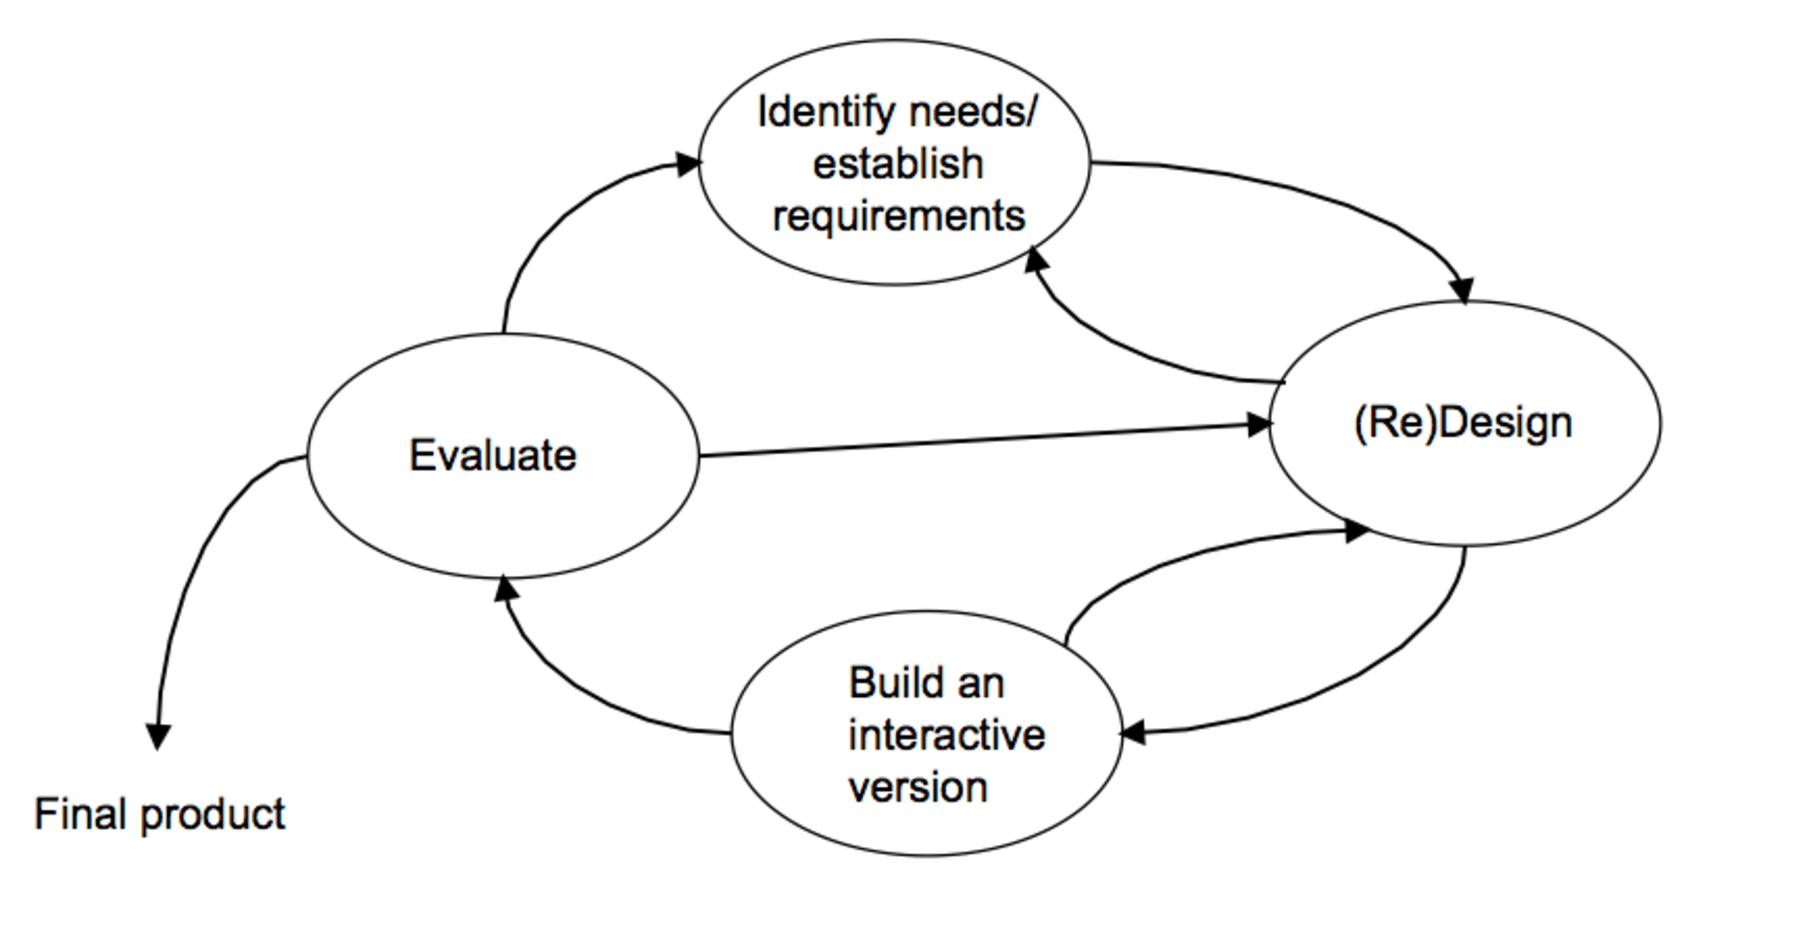
\includegraphics[width=0.8\textwidth]{images/method/UCD.pdf}
	\caption{User Centered Design Process TODO MATTHIAS QUELLE ANGEBEN!}
	\label{fig:UCD}
\end{figure}

During the \emph{Research Phase} information about the users, their profiles and their needs is collected. During the \emph{Design Phase} the requirements are specified based on the information gathered in the research phase and the concepts are created. During the \emph{Prototyping Phase} various forms of mockups and prototypes are created based on the information gathered in the design phase. In the \emph{Evaluation Phase} the prototypes and mockups are finally discussed with the users and evaluated. It is important to repeatedly check if the needs of the users are still met. Therefore the phases are interconnected and fast iteration is a vital part of User Centered Design.

\subsection{Experimental Horizontal Prototyping}
We decided for a combination of experimental and horizontal prototyping as software development method.

Experimental prototyping aims at creating a prototype of the system in an early phase of the development process and is therefore highly compatible with the use of user centered design (see \ref{subsect:ucd}).
There is also a connection to the empirical study part (see \ref{subsect:emp_study}), as the prototype shall be used for evaluating requirements of users as well as of partners from the industry. Not only should an early prototype lead to a higher-sophisticated user interface with respect to ui design principles and usability issues, but also provide possibility to gain results for the research part of the overall project. 

The prototyping shall be executed in a horizontal manner, that means there should be a fully designed user interface before starting over with any kind of business logic implementation. In contrast to that, vertical prototyping aims at implementing one specific feature from the frontend to the backend with its full functionality. The advantage of an horizontal approach is, similar to an experimental one, the perfect compatibility with user centered design. Of course this requires a strict separation of user interface and business logic implementation. See figure \ref{fig:prototyping} for a distinction between horizontal and vertical prototyping.

\begin{figure}[htb]
	\centering
		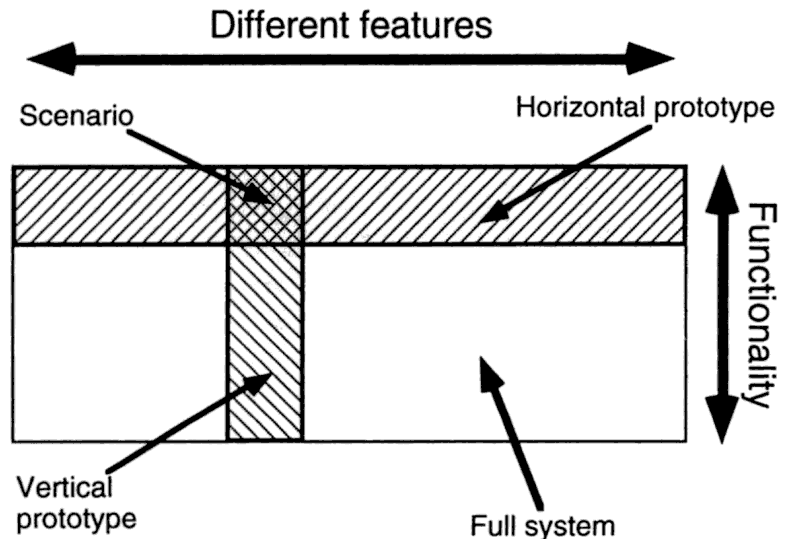
\includegraphics[width=0.6\textwidth]{images/method/prototyping}
	\caption{Horizontal and vertical prototyping \citep[Page 94]{DBLP:books/daglib/0076830}}
	\label{fig:prototyping}
\end{figure}

One advantage of prototyping is that potential errors in the user interface can be detected in an early phase of the project - also quality assurance can get embedded into the project as early as possible.

\subsection{Empirical Study}
\label{subsect:emp_study}

Empirical study of the needs of the main stakeholders in the project is essential. By means of surveys and interviews we try to identify requirements and hope to get answers to the following (and more) questions:

\begin{itemize}
\item What do end users need/want? What is negligible and can therefore be omitted?
\item What do they miss in actual systems?
\item How do they wish to interact with the system?
\item What are the needs of the different business partners?
\item Which systems are currently in use at the partners processes?
\item How would they improve their current systems?
\end{itemize}

Of course empirical study has to take place at a very early phase in the project to prevent undesirable development and ensure movement into the right direction from the very beginning. The contents of the questionnaire therefore have to be prepared conscientiously and meaningful, so that as much findings as possible can be deduced for use in later phases of the project.

\subsection{Literature Research}

Certainly we do not have to reinvent the wheel. Therefore a detailed literature research has to be carried out to find possible approaches that can be reused. By finding other scientific work at the same topics we want to save both time and unnecessary work that has already been done by others projects. The literature research part aims at answering the following questions

\begin{itemize}
\item Which techniques are already in use or have been introduced in the field of
\begin{itemize}
\item healthcare applications?
\item ubiquitous systems?
\item user centered design?
\item usability engineering?
\item ...
\end{itemize}
\item Which of the found techniques can be reused?
\item What can be improved?
\end{itemize}

%\note{
%\begin{itemize}
%\item {\em Length: 2-5 pages}
%\item {\bf How?}
%\item How should the expected results be achieved?
%\item What method(s) will be applied? (e.g., empirical study, user-centered design, prototype implementation,...)
%\item Description of the methods.
%\item Justifications for chosen methods.
%\end{itemize}
%}

% --------------------------------------------------------------
\newpage
\section{Detailed description of the workpackages}
\label{sect:workplan}

%\note{
%\begin{itemize}
%\item {\em Length: 2-4 pages}
%\item Structuring the project into self-contained parts.
%\item Additional verbal descriptions.
%\item Work packages
%    \begin{itemize}
%    \item title
%    \item goal(s)
%    \item description
%    \item expected results
%    \item responsible person(s)
%    \item dependencies
%    \end{itemize}
%\end{itemize}
%}

\subsection{Phase: Range of Functions}
\label{sect:workplan:rangeoffucntions}

\subsubsection{Literature Research LR1}
\label{sect:workplan:phase1:lr1}
\textbf{Dependencies:} None\\
\textbf{Description:} Find and describe existing Systems and emphasis their approach.
Analyze the user-interfaces and the provided interaction with the system. Establish the functionality and their business model.\\
\textbf{Responsible person(s):} Research Group\\
\textbf{Goal(s) and expected Results:} Information about current systems, their feature set and user-interface\\

\subsubsection{Empirical Study ES1}
\label{sect:workplan:phase1:es1}
\textbf{Dependencies:} LR1 \ref{sect:workplan:phase1:lr1}\\
\textbf{Description:} Create questionary for users, to get information about their thoughts about the systems discovered in \ref{sect:workplan:phase1:lr1}. They should evaluate these results and discover issues with their User-Interface and functionality and also mention their needs regarding these two aspects.\\
The users current situation regarding the usage or the willingness to use of current systems are also parts to work out. \\
\textbf{Responsible person(s):} Research Group, Alpha-User \\
\textbf{Goal(s) and expected Results:} Knowledge about the user needs.\\

\subsubsection{Empirical Study ES2}
\label{sect:workplan:phase1:es2}
\textbf{Dependencies:} LR1 \ref{sect:workplan:phase1:lr1}\\
\textbf{Description:} Meeting with possible service partners (restaruants, supermarkets, doctors, etc.) to identify their currently used systems and their needs, thoughts and whishes and specify how a cooperation could look like.\\
\textbf{Responsible person(s):} Strategy Team\\
\textbf{Goal(s) and expected Results:} Knowledge about the needs of service partners. Signed partner contracts. \\

\subsubsection{Range of Functions RF1}
\label{sect:workplan:phase1:rf1}
\textbf{Dependencies:} LR1 \ref{sect:workplan:phase1:lr1}\\
\textbf{Description:} Brainstorming about possible features of the system using knowledge discovered during step LR1 (\ref{sect:workplan:phase1:lr1}).\\
\textbf{Responsible person(s):} Research Team\\
\textbf{Goal(s) and expected Results:} Possible feature list\\

\pagebreak
\subsubsection{Range of Functions RF2}
\label{sect:workplan:phase1:rf2}
\textbf{Dependencies:} RF1 \ref{sect:workplan:phase1:rf1}, ES1 \ref{sect:workplan:phase1:es1}, ES2 \ref{sect:workplan:phase1:es2}\\
\textbf{Description:} Combine knowledge from the two empirical studies ES1 and ES2 and evaluate the brainstormed feature list. Check if the discovered features from the empirical studies are matching the created feature list\\
\textbf{Responsible person(s):} Research Team\\
\textbf{Goal(s) and expected Results:} Final set of features for version 1.0 (Milestone M1)\\

\subsection{Phase: Towards Release}
\label{sect:workplan:towardsrelease}

\subsubsection{Prototyping P1}
\label{sect:workplan:phase2:p1}
\textbf{Dependencies:} RF2 \ref{sect:workplan:phase1:rf2}\\
\textbf{Description:} Create first version of horizontal prototype by creating the user-interface. Every part of the system should be covered.\\
\textbf{Responsible person(s):} Dev-Team\\
\textbf{Goal(s) and expected Results:} first version of prototype\\

\subsubsection{Evaluation and Redesign ER1}
\label{sect:workplan:phase2:er1}
\textbf{Dependencies:} P1 \ref{sect:workplan:phase2:p1}\\
\textbf{Description:} The Alpha-Users should evaluate the prototype (interface and interaction) and redesign it by taking care of their input. This step should be repeated several times until there is no more additional useful feedback from the user-group.\\
\textbf{Responsible person(s):} Research-Group, Alpha-Users, Dev-Team\\
\textbf{Goal(s) and expected Results:} Information about necessary changes and redesigned prototype\\

\subsubsection{Prototyping P2}
\label{sect:workplan:phase2:p2}
\textbf{Dependencies:} P1 \ref{sect:workplan:phase2:p1}\\
\textbf{Description:} Extend the existing prototype by adding functionality and implement the features.\\
\textbf{Responsible person(s):} Dev-Team\\
\textbf{Goal(s) and expected Results:} Prototype with all features\\

\pagebreak
\subsubsection{Evaluierung und Redesign ER2}
\label{sect:workplan:phase2:er2}
\textbf{Dependencies:} P2 \ref{sect:workplan:phase2:p2}, ER2 \ref{sect:workplan:phase2:er2}\\
\textbf{Description:} The new prototype should be reevaluated by the Alpha-Users and also from the Dev-Team (including Security and Quality Specialists). This step covers not only the interface and interaction, but also the quality and security of the product. The knowledge should be used to redesign the prototype and this step should be repeated several times. After a number of iterations the status of the web application should be switched to Beta and Beta-Users will be able to sign in and use the systems. After the last iteration the status should be switched to Release.\\
\textbf{Responsible person(s):} Alpha-Users, Beta-Users, Strategy Team, Dev-Team\\
\textbf{Goal(s) and expected Results:} Released web application (Milestone M2)\\

\subsection{Phase: Connect to 3rd Party Services and mobile Client}
\label{sect:workplan:3rdpartiesandmobileclient}

\subsubsection{Literature Research LR2}
\label{sect:workplan:phase3:lr2}
\textbf{Goal(s):} \\
\textbf{Dependencies:} \\
\textbf{Description:} \\
\textbf{Responsible person(s):} \\
\textbf{Expected Results:} \\

\subsubsection{Empirical Studie ES3}
\label{sect:workplan:phase3:es2}
\textbf{Goal(s):} \\
\textbf{Dependencies:} \\
\textbf{Description:} \\
\textbf{Responsible person(s):} \\
\textbf{Expected Results:} \\

\subsubsection{Range of Function RF2}
\label{sect:workplan:phase3:rf2}
\textbf{Goal(s):} \\
\textbf{Dependencies:} \\
\textbf{Description:} \\
\textbf{Responsible person(s):} \\
\textbf{Expected Results:} \\

\subsubsection{Range of Function RF3}
\label{sect:workplan:phase3:rf3}
\textbf{Goal(s):} \\
\textbf{Dependencies:} \\
\textbf{Description:} \\
\textbf{Responsible person(s):} \\
\textbf{Expected Results:} \\

\subsubsection{Prototyping P3}
\label{sect:workplan:phase3:p3}
\textbf{Goal(s):} \\
\textbf{Dependencies:} \\
\textbf{Description:} \\
\textbf{Responsible person(s):} \\
\textbf{Expected Results:} \\

\subsubsection{Evaluierung und Redesign ER3}
\label{sect:workplan:phase3:er3}
\textbf{Goal(s):} \\
\textbf{Dependencies:} \\
\textbf{Description:} \\
\textbf{Responsible person(s):} \\
\textbf{Expected Results:} \\


% --------------------------------------------------------------
\pagebreak
\section{Time plan (Gantt chart)}
\label{sect:timeplan}

\note{
\begin{itemize}
\item {\em Length: 1-2 pages}
\item Realistic estimation of schedule based on workpackages.
\item Including milestones (not only when but also what is to be achieved for each milestone).
\item Generation of a Gantt chart. (Including phases, milestones, buffer times, critical areas, etc.)
\end{itemize}
}

% --------------------------------------------------------------
\section{Human resources / team}
\label{sect:team}

\note{
\begin{itemize}
\item {\em Length: 1-2 pages}
\item Description of the team that is needed to carry out the project. (For the execution phase of the project, not the planning phase.)
\item How many people?
\item To what extent are individual members needed?
\item What knowledge, skills, and experiences are needed for each member?
\item Demonstrate that the members will be able to carry out the project successfully.
\item Work structure
	\begin{itemize}
	\item     Who will lead the project?
	\item     How do they work together?
	\item     Management and coordination
		\begin{itemize}
		\item 	        What communication structures will be established? (e.g., mailing list, blog, CMS, CVS, ...)
		\item 	        How often will meetings take place? (Who will participate?)
		\item 	        How will the work be documented?
		\item 	        How will information be stored and shared?
		\end{itemize}
	\end{itemize}
\item Cooperations
	\begin{itemize}
	\item     Will external cooperators be part of the project? (e.g., other research institutions or companies)
	\item     What is their role?
	 \item    Why are they needed?
	\end{itemize}
\end{itemize}
}

% --------------------------------------------------------------
\section{Costs}
\label{sect:costs}

\note{
\begin{itemize}
\item {\em Length: 2-3 pages}
\item Rough estimation of cost in form of calculation (table(s)) + descriptive text.
\item Justification for the personnel and non-personnel costs (equipment, material, travel and other costs)
\item An Excel template is provided as supplementary material to support budgeting.
\item Personnel costs
	\begin{itemize}
	\item     Justification for the personnel to be assigned to the project (type of position(s), description of nature of work, length and extent of involvement in the project)
	\item     The application should include all persons who will be required for the proposed project (project lead, researchers, developers, advisory board, etc.). The available legal categories of employment are contracts of employment for full- or part-time employees (DV) and reimbursement for work on an hourly basis (GB). In addition, a part-time contract of employment (DV 50\%, ``studentische Mitarbeiter'') may be requested for people who have not yet completed a Master or Diploma program (Diplom) in the relevant subject.
	 \item    The justification of the requested personnel should contain:
		\begin{itemize}
		\item 	        description of type of work;
		\item 		        extent of involvement (part-time contracts are permitted).
		\end{itemize}
	\item Exact numbers of employment categories can be found on the FWF Website (\href{http://www.fwf.ac.at/de/projects/personalkostensaetze.html}{http://www.fwf.ac.at/de/projects/personalkostensaetze.html})
	\end{itemize}
\item Equipment costs
	\begin{itemize}
	\item     Indicate reasons for equipment costs. The ``scientific equipment'' category includes instruments, system components, costs for the use of software required by the project and other durable goods provided the cost per item (including VAT) exceeds EUR 1,500.00.
	\end{itemize}
\item Material costs
	\begin{itemize}
	\item     This category encompasses consumables and smaller pieces of equipment where the cost per item is below EUR 1,500.00 including VAT. The calculation of requested material costs should be justified with reference to the schedule, work plan and experimental plan. Experience with previous projects should be taken into account.
	\end{itemize}
\item Travel costs
	\begin{itemize}
	\item     Funding may be requested for the costs of project-specific travel and accommodation, field work, expeditions, etc. Applicants are to provide a detailed travel (cost) plan broken down by project participant. For brief stays, the calculation of the travel and accommodation costs should be based on the federal regulations governing travel costs (RGV). The RGV rates governing Austria and abroad may be found in the FAQs on the FWF Website (\href{http://www.fwf.ac.at/de/faq/reisegebuehrenvorschrift.html}{http://www.fwf.ac.at/de/faq/reisegebuehrenvorschrift.html}). For longer stays an appropriate and comprehensible cost plan should be prepared.
	\end{itemize}
\item Other costs
	\begin{itemize}
	\item     Independent contracts for work and services (costs for work of clearly defined scope and content assigned to individuals, provided that this is scientifically justifiable and economical)
    	\item     Costs that cannot be included under personnel, equipment, material or travel costs, such as:
		\begin{itemize}
		\item         reimbursement of costs towards or for the use of research facilities, e.g. of large-scale research facilities (project-specific 'equipment time'). Applicants should obtain and submit multiple offers;
		\item         costs for project-specific work carried out outside the applicant's research institution (e.g. for analysis work performed elsewhere, for interviews, for sample collection, for preparation of thin slices etc.). Applicants should obtain and submit multiple offers;
		\item         honoraria for test persons;
		\end{itemize}
	\end{itemize}
\end{itemize}
}

% --------------------------------------------------------------
\section{Expected implications and risks}
\label{sect:implication-risk}

\note{
\begin{itemize}
\item {\em Length: 1-2 pages}
\item Importance of the expected results for the discipline
	\begin{itemize}
	\item     To what extent does the proposed research address important challenges?
	\end{itemize}
\item Importance of the expected results for other areas
\item What are possible risks of the project and how can they be alleviated?
	\begin{itemize}
	\item     What factors could lead to a failure of the project?
	\item     Which factors or persons could support the project and increase the chance for success?
	\item     What if important team members leave the project?
	\end{itemize}
\end{itemize}
}

% --------------------------------------------------------------
\section{Ethical considerations \& security issues}
\label{sect:ethics-security}

\note{
\begin{itemize}
\item {\em Length: 1-2 pages}
\item Provide a brief explanation of the ethical issue involved and how it will be dealt with appropriately.
\item Are there any security-sensitive issues that apply to your proposal?
\end{itemize}
}

% --------------------------------------------------------------
% APPENDIX
\begin{appendix}

\pagebreak

% --------------------------------------------------------------
% References
\phantomsection
\addcontentsline{toc}{section}{References}

\bibliographystyle{plainnat}
\nocite{*}

\bibliography{mswp2012-proposal}

\pagebreak

% --------------------------------------------------------------
% Abbreviations
\section*{Abbreviations}
 \addcontentsline{toc}{section}{Abbreviations}
 
 \begin{description}
  \item[MSWP] Management von Software Projekten
  \item[WP] Work Package
  \item[OECD] Organisation for Economic Co-operation and Development
  \item[RKI] Robert Koch Institut
 \end{description}

\end{appendix}


\end{document}
